\documentclass[border=10pt]{standalone}
\usepackage{tikz}
\begin{document}
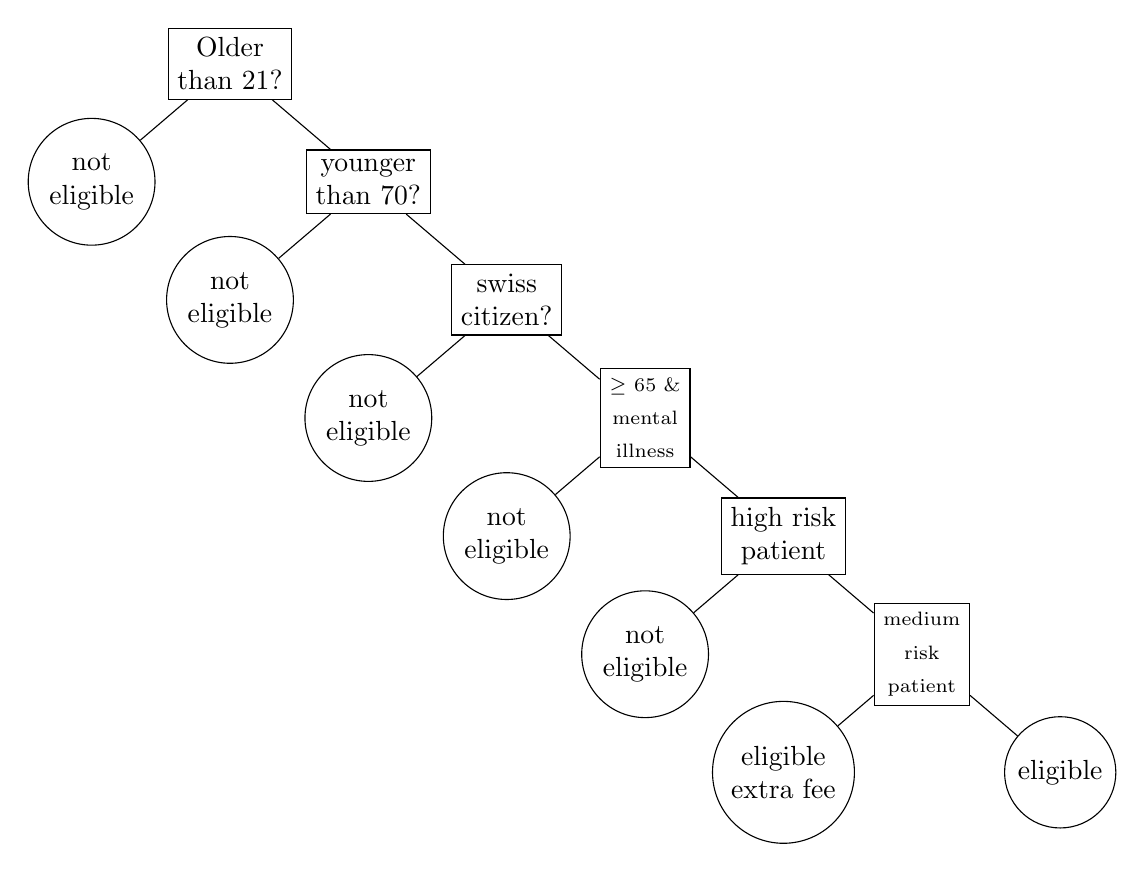
\begin{tikzpicture}[sibling distance=10em,
  every node/.style = {shape=rectangle,
    draw, align=center}]]


  \node {Older\\than 21?}
    child { node[circle] {not\\eligible} }
    child { node {younger\\than 70?}
      child { node[circle] {not\\eligible} }
      child { node {swiss\\citizen?}
        child { node[circle] {not\\eligible}}
        child { node {\scriptsize\(\geq\) 65 \& \\ \scriptsize mental\\\scriptsize illness}
            child { node[circle] {not\\eligible}}
            child { node {high risk\\patient}
                child { node[circle] {not\\eligible}}
                child { node {\scriptsize medium\\\scriptsize risk\\\scriptsize patient}
                    child { node[circle] {eligible\\extra fee}}
                    child { node[circle] {eligible}}
                }
            }
        }
      } };
\end{tikzpicture}
\end{document}